\documentclass[border=10pt]{standalone}
\usepackage{pgfplots}
\pgfplotsset{compat=1.18}
\begin{document}
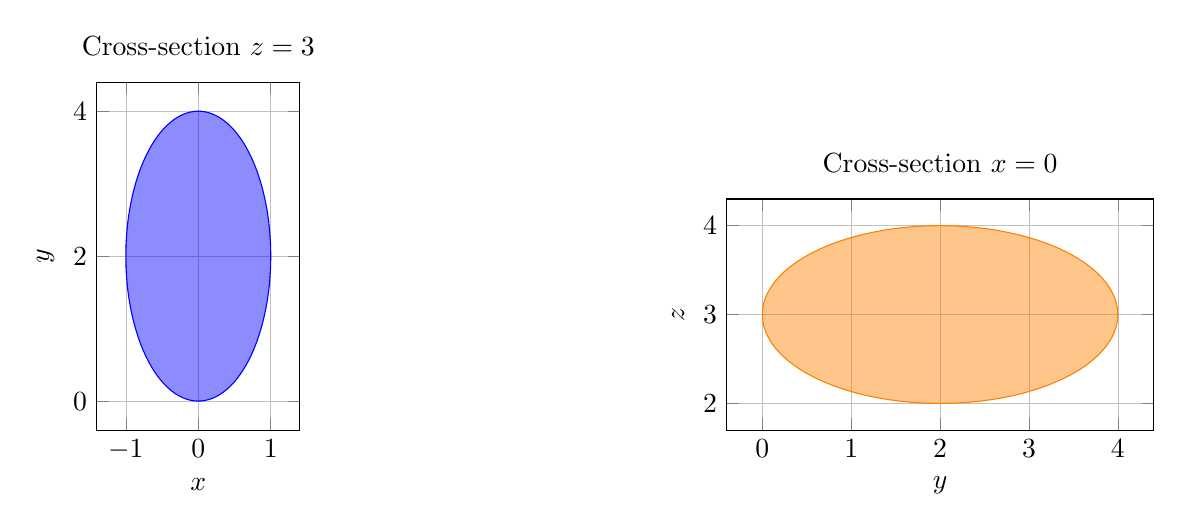
\begin{tikzpicture}
\begin{axis}[
  width=7cm, height=6cm,
  axis equal image,
  xmin=-1.4, xmax=1.4, ymin=-0.4, ymax=4.4,
  xlabel={$x$}, ylabel={$y$},
  title={Cross-section $z=3$},
  grid=both,
  grid style={line width=.1pt, draw=gray!30},
  major grid style={line width=.2pt, draw=gray!50},
  enlarge x limits=false,
  enlarge y limits=false
]
\addplot[domain=0:360, samples=120, fill=blue, fill opacity=0.45, draw=blue]
  ({cos(x)}, {2+2*sin(x)}) -- cycle;
\end{axis}

\begin{axis}[
  width=7cm, height=6cm,
  at={(8cm,0)},
  axis equal image,
  xmin=-0.4, xmax=4.4, ymin=1.7, ymax=4.3,
  xlabel={$y$}, ylabel={$z$},
  title={Cross-section $x=0$},
  grid=both,
  grid style={line width=.1pt, draw=gray!30},
  major grid style={line width=.2pt, draw=gray!50},
  enlarge x limits=false,
  enlarge y limits=false
]
\addplot[domain=0:360, samples=120, fill=orange, fill opacity=0.45, draw=orange]
  ({2+2*cos(x)}, {3+sin(x)}) -- cycle;
\end{axis}
\end{tikzpicture}
\end{document}